% ============================================================
%  Fanteng Meng — Curriculum Vitae
%  Compiled with pdflatex
% ============================================================
\documentclass[11pt,a4paper]{article}

% ---- Packages ----
\usepackage[margin=0.85in]{geometry}
\usepackage[utf8]{inputenc}
\usepackage[T1]{fontenc}
\usepackage{mathpazo}              % Palatino-like serif
\usepackage[scaled=0.88]{helvet}   % Sans-serif for headings
\usepackage{enumitem}
\usepackage{titlesec}
\usepackage{xcolor}
\usepackage{hyperref}
\usepackage{tabularx}
\usepackage{graphicx}              % For photo

% ---- Colors ----
\definecolor{sectioncolor}{RGB}{0,51,145}
\definecolor{accent}{RGB}{100,80,155}
\definecolor{graytext}{RGB}{100,100,100}
\definecolor{linkcolor}{RGB}{60,80,160}

% ---- Hyperlinks ----
\hypersetup{
  colorlinks=true,
  linkcolor=linkcolor,
  urlcolor=linkcolor,
  pdftitle={Fanteng Meng -- CV},
  pdfauthor={Fanteng Meng}
}

% ---- Section formatting ----
\titleformat{\section}
  {\sffamily\bfseries\large\color{sectioncolor}}
  {\thesection}{1em}{}[\vspace{-3pt}\textcolor{sectioncolor}{\rule{\textwidth}{0.6pt}}\vspace{-6pt}]
\titlespacing*{\section}{0pt}{14pt}{8pt}

\titleformat{\subsection}
  {\sffamily\bfseries\color{sectioncolor}}
  {\thesubsection}{1em}{}
\titlespacing*{\subsection}{0pt}{8pt}{2pt}

% ---- Custom environments ----
\newenvironment{entrylist}
  {\begin{itemize}[leftmargin=*,nosep,itemsep=2pt]}
  {\end{itemize}}

\newlength{\datelabelwidth}
\newcommand{\cvitem}[3]{%
  \setlength{\datelabelwidth}{2.8cm}%
  \noindent%
  \parbox[t]{\datelabelwidth}{\raggedleft\footnotesize\sffamily\color{graytext}#1}%
  \hspace{0.6cm}%
  \parbox[t]{\dimexpr\textwidth-\datelabelwidth-0.6cm\relax}{%
    \textbf{#2}\par\small#3\par}%
  \vspace{2.5mm}\par%
}

% ---- Header ----
\newcommand{\makecvheader}{%
  \noindent
  \begin{minipage}[t]{3.4cm}
    \vspace{0.1em}
    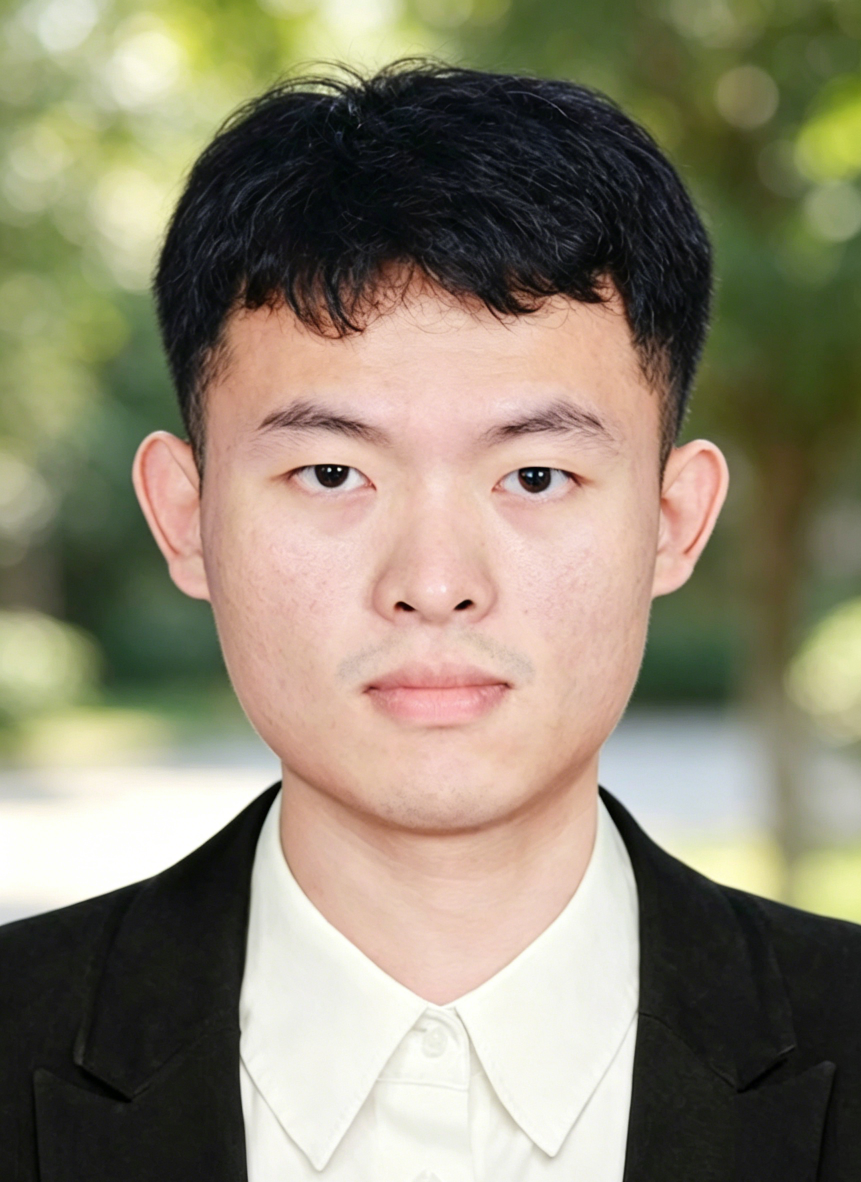
\includegraphics[width=3.15cm,height=3.15cm,keepaspectratio,clip]{../images/photo-202601-square.png}%
  \end{minipage}\hspace{1.2em}%
  \begin{minipage}[t]{0.60\textwidth}
    \vspace{0.7em}
    {\fontsize{22}{26}\selectfont\sffamily\bfseries Fanteng Meng}\par
    \vspace{1pt}\color{graytext}\large Ph.D.\ Student in Safety Science \& Engineering\par
    \vspace{6pt}\small
    \href{mailto:ftmeng@bjtu.edu.cn}{ftmeng@bjtu.edu.cn}\,
    $\cdot$\,
    \href{https://ft115.github.io}{ft115.github.io}\,
    $\cdot$\,
    \href{https://scholar.google.com.hk/citations?user=Yq5wnc8AAAAJ}{Google Scholar}\par
    \vspace{3pt}\footnotesize\color{graytext}State Key Laboratory of Rail Traffic Control and Safety, Beijing Jiaotong University\\[1pt]
    \footnotesize\color{graytext}Transportation College, Beijing Jiaotong University, Beijing, China
  \end{minipage}
  \par\vspace{3pt}
  \noindent\textcolor{black}{\rule{\textwidth}{0.4pt}}\vspace{5pt}
}

\begin{document}
\emergencystretch=2.5em
\widowpenalty=10000
\clubpenalty=10000
\brokenpenalty=10000
\displaywidowpenalty=10000

\makecvheader

% ============================================================
\section{Education}

\cvitem{2023 -- Present}
  {Ph.D., Safety Science \& Engineering}
  {Beijing Jiaotong University (BJTU), State Key Lab of Rail Traffic Control \& Safety \&\\
   Transportation College (Intelligent Systems Dept.)\\
   Advisor: Prof.~Yong Qin\\
   Enrolled via successive master-doctor program since 2023.}

\cvitem{2022 -- 2023}
  {M.Eng., Transportation Planning \& Management}
  {Beijing Jiaotong University (BJTU)}

\cvitem{2018 -- 2022}
  {B.Eng., Transportation}
  {Shijiazhuang Tiedao University}

% ============================================================
\section{Research Interests}

\noindent
UAV-based intelligent inspection; Machine vision \& deep learning for rail transit;
Edge computing; 3D reconstruction \& point cloud analysis;
Full-stack low-altitude intelligent perception systems.

% ============================================================
\section{Research Projects}

{\footnotesize\color{graytext}P.I. for the item marked (P.I.); the rest are core participants (Core).}

\begin{enumerate}[leftmargin=1.6em,itemsep=2.5pt]
  \item \textbf{Development and Demonstration Verification of Safety-Guarantee Technologies for Autonomous Rail Transit Systems.} (2022--2026) -- National Key R\&D Program (Core)
  \item \textbf{Research on Unknown-Risk Identification of High-Speed Railway Surroundings from UAV Remote Sensing Imagery.} (2024--2026) -- Fundamental Research Funds for the Central Universities (P.I.)
  \item \textbf{In-depth Research and Application of UAV Inspection Technology for High-Speed Railway Infrastructure.} (2022--2024) -- China Railway ``Major Project'' (Core)
  \item \textbf{Construction of an Automatic UAV Intelligent Inspection System for Beijing--Shanghai HSR Infrastructure.} (2023--2024) -- Beijing--Shanghai HSR ``Major Project'' (Core)
  \item \textbf{Research on Automated Overhaul Equipment and Key Technologies for Railway Steel-Truss-Bridge Coating.} (2024--2027) -- Beijing--Shanghai HSR ``Major Project'' (Core)
  \item \textbf{Application of Autonomous-UAV Inspection to Defects and Rockfall Debris in Key Zones of Qinghai--Tibet Railway Bridges.} (2026--2027) -- ``Smart Sky Road'' Major Project of the Qinghai--Tibet Railway (Core)
\end{enumerate}

% ============================================================
\section{Selected Publications}

\noindent\textit{* Corresponding author \quad $^\#$ Co-first author}

\begin{enumerate}[leftmargin=*,nosep,itemsep=1.5pt]
  \item \textbf{Meng, F.}, Qin, Y.$^*$, Wu, Y.$^*$, et al.\
    ``SRLF: Sparse Representation Learning Framework for Railroad Surrounding Potential Risk Perception Using UAV Imagery.''
    \textit{IEEE Trans.\ Intell.\ Transp.\ Syst.}, 2025.

  \item \textbf{Meng, F.}, Qin, Y.$^*$, Wu, Y.$^*$, Shao, C., Yang, H., Jia, L.\
    ``Automatic Risk Level Evaluation System for Potential Environmental Hazards along High-speed Railroad Using UAV Aerial Photograph.''
    \textit{Expert Syst.\ Appl.}, 2025.

  \item \textbf{Meng, F.}, Qin, Y.$^*$, Wu, Y.$^*$, Shao, C., Jia, L.\
    ``A Subtle Defect Recognition Method for Catenary Fastener in High-speed Railroad Using Destruction and Reconstruction Learning.''
    \textit{Adv.\ Eng.\ Inform.}, 2024.

  \item Wu, Y.$^\#$, \textbf{Meng, F.}$^\#$, Qin, Y.$^*$, Qian, Y.$^*$, Xu, F., Jia, L.\
    ``UAV Imagery Based Potential Safety Hazard Evaluation for High-speed Railroad Using Real-time Instance Segmentation.''
    \textit{Adv.\ Eng.\ Inform.}, 2023.

  \item Wu, Y.$^\#$, \textbf{Meng, F.}$^\#$, Qin, Y.$^*$, Qian, Y.$^*$, Liu, Z., Zhao, W.\
    ``Automated Anomaly Detection of Catenary Split Pins Using Unsupervised Learning.''
    \textit{Autom.\ Constr.}, 2024.

  \item \textbf{Meng, F.}, Qin, Y.$^*$, Cui, J., Wu, Y., Zhang, Z., Wei, S.\
    ``Unknown Risk Detection in External Environment of Railroad Using UAV Images.''
    \textit{Acta Aeronaut.\ Astronaut.\ Sin.}, 2025.

  \item Qin, Y.$^*$, \textbf{Meng, F.}$^\#$, Zhang, Z., et al.\
    ``Autonomous UAV-based Intelligent Inspection Framework for Rail Transit Infrastructure: A Review.''
    \textit{J.\ Beijing Jiaotong Univ.}, 2025.
\end{enumerate}

% ============================================================
\section{Selected Engineering Projects}

\begin{enumerate}[leftmargin=*,nosep,itemsep=4pt]

  \item \textbf{Fully-automatic UAV Intelligent Inspection System for High-speed Railway}
  \begin{itemize}[leftmargin=*,nosep]
    \item Core researcher in national key R\&D program; designed 3 vision algorithms (\textgreater{}96\% recall).
    \item Deployed 6 UAVs + 4 auto drone nests; achieved 10$\times$ efficiency gain over manual inspection.
  \end{itemize}

  \item \textbf{UAV Inspection for Bridges \& Rockfall Hazards, Qinghai-Tibet Railway}
  \begin{itemize}[leftmargin=*,nosep]
    \item Full-stack R\&D: autonomous flight control, photogrammetry 3D reconstruction, point cloud segmentation.
    \item Multi-temporal registration \& rockfall deformation detection for plateau railway safety.
  \end{itemize}

  \item \textbf{Full-coverage UAV Inspection \& Coating Defect Evaluation for Railway Steel Truss Bridge}
  \begin{itemize}[leftmargin=*,nosep]
    \item Designed obstacle-avoidance flight modes covering top, side, \& under-bridge zones.
    \item End-to-end workflow: coating defect recognition $\to$ quantitative grading $\to$ spatial traceability.
  \end{itemize}

\end{enumerate}

% ============================================================
\section{Patents}

\noindent\textbf{Granted Patents}

\begin{enumerate}[leftmargin=*,nosep,itemsep=2pt]
  \item Autonomous UAV Based Intelligent Inspection System for Equipment, Facilities, and the Environment along Railway Lines and Method Thereof. (US Patent)
  \item Railway Environmental Hazard Identification and Risk Level Assessment Method Based on UAV Images.
  \item UAV Route Generation Method for Transportation Facility Inspection under GNSS-denied Environments.
  \item Cross-modal Adaptive Matching Based Online Extrinsic Calibration Method and System for LiDAR and Camera.
\end{enumerate}

\noindent\textbf{Published Patent Applications}

\begin{enumerate}[leftmargin=*,nosep,itemsep=2pt]
  \item Refined Catenary Split Pin Defect Recognition Method for Railway Catenary.
  \item Coating Corrosion Detection, Assessment Method and System for Railway Steel Truss Bridges.
  \item Unknown Risk Identification Method for Railway Surrounding Environment Using UAV Remote Sensing Images.
\end{enumerate}

% ============================================================
\section{Honors \& Awards}

\begin{itemize}[leftmargin=*,nosep,itemsep=2pt]
  \item[2024] Leading Technology Award (Outstanding Achievement), World Internet Conference --- ``Fully-autonomous UAV Intelligent Inspection Technology and Application for Rail Transit''
  \item[2024] Silver Award, 14th Challenge Cup National College Students' Entrepreneurship Competition (Belt \& Road Intl.\ Invitational)
  \item[2024] Silver Award, ``Qingchuang Beijing'' Capital College Students Challenge Cup Entrepreneurship Competition
  \item[2022] Second Place, Beijing Jiaotong University Summer Deep Learning Championship
  \item[2021] First Prize, China Transportation Outstanding Student Award
  \item[2021] Provincial First Prize, 7th National College Students Engineering Training Integration Ability Competition
  \item[2021] Provincial Merit Student
  \item[2020] Provincial First Prize, 12th National College Students Mathematics Competition
  \item[2020] Provincial First Prize, 7th College Students Physics Competition
\end{itemize}

% ============================================================
\section{Professional Service}

\noindent\textbf{Journal Reviewer}\quad
\textit{IEEE Trans.\ Intell.\ Transp.\ Syst.} (T-ITS),
\textit{Adv.\ Eng.\ Inform.} (AEI),
\textit{Expert Syst.\ Appl.} (ESWA)

% ============================================================
\section{Technical Skills}

\noindent
\textbf{Languages:}\ \ Python, C++, Matlab
\quad
\textbf{Deep Learning:}\ \ PyTorch
\quad
\textbf{Systems:}\ \ Linux, ROS
\quad
\textbf{Vision:}\ \ OpenCV
\quad
\textbf{Hardware:}\ \ DJI-PSDK

\end{document}